\subsection{Templated UIComponent}
While creating the GUI library, we've used a lot of templating. This was done 
so that we can reuse our templated GUI classes if and when we decide to 
switch to OpenGL. The lowest level GUI class is called the UIComponent, 
which has a couple of template parameters for which rendering engine we're 
using,  the type of data its rendering object (see \cref{sec:rendering-ui} for 
an explanation about how the UIComponents get rendered.) contains, what kind 
of data it returns when rendering and the type of data for its mouse callback 
object (which will be explained in \cref{sec:eventhandling}).

The UIComponent class can be seen in \cref{fig:uicomponent}.

\begin{figure}[H]
\centering
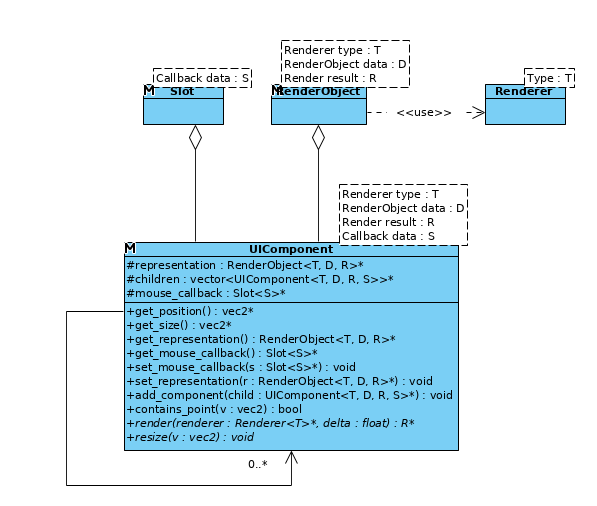
\includegraphics[scale=0.55]{res/ui/uicomponent.png}
\caption{UIComponent class.}\label{fig:uicomponent}
\end{figure}

